\documentclass{ximera}

\newcommand{\RR}{\mathbb R}
\renewcommand{\d}{\,d}
\newcommand{\dd}[2][]{\frac{d #1}{d #2}}
\renewcommand{\l}{\ell}
\newcommand{\ddx}{\frac{d}{dx}}
\newcommand{\dfn}{\textbf}
\newcommand{\eval}[1]{\bigg[ #1 \bigg]}


\author{Bart Snapp
}
\license{Creative Commons 4.0 By-SA}

\begin{document}
\textbf{For problems 1--4,} use table of \textbf{gradient vectors} for the
function $F:\R^2\to\R$ given below:
\begin{image}
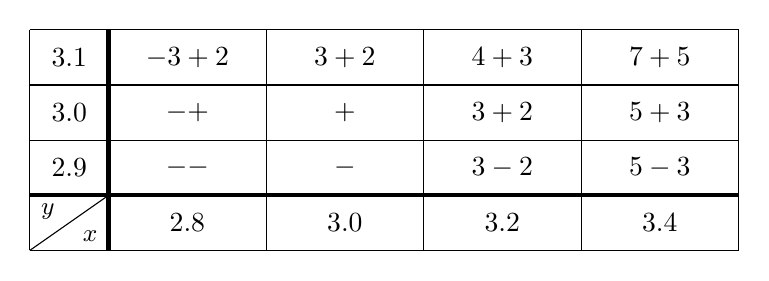
\begin{tikzpicture}[x=1cm,y=.7cm]

  %% \draw[fill=white!80!black]
  %% (1,2) -- (5,2) --(5,4) -- (3,4) -- (3,3) -- (1,3)--cycle;%(3,3) -- (7,3) --(7,2) -- (3,2)--cycle;
  
  \draw (0,0) grid [step=1] (1,4);
  \draw (3,4) -- (3,0);
  \draw (5,4) -- (5,0);
  \draw (7,4) -- (7,0);
  \draw (9,4) -- (9,0);
  
  \draw (0,0) -- (9,0);
  \draw (0,1) -- (9,1);
  \draw (0,2) -- (9,2);
  \draw (0,3) -- (9,3);
  \draw (0,4) -- (9,4);


  
  \draw[ultra thick] (0,1)--(9,1);
  \draw[ultra thick] (1,4)--(1,0);
  
  \draw (0,0) -- (1,1);
  %\node at (.9,.9) [below left,inner sep=1pt] {\small$y$};
  %\node at (0.1,.1) [above right,inner sep=1pt] {\small$x$};
  \node at (.1,.9) [below right,inner sep=1pt] {\small$y$};
  \node at (0.9,.1) [above left,inner sep=1pt] {\small$x$};
  
  
  %% x-values
  \node at (2,.5) {$2.8$};
  \node at (4,.5) {$3.0$};
  \node at (6,.5) {$3.2$};
  \node at (8,.5) {$3.4$};
  
  %% y-values
  \node at (0.5,1.5) {$2.9$};
  \node at (0.5,2.5) {$3.0$};
  \node at (0.5,3.5) {$3.1$};
  
  
  %% vectors
  %% top row
  \node at (2,3.5) {$-3\veci+2\vecj$};
  \node at (4,3.5) {$3\veci+2\vecj$};
  \node at (6,3.5) {$4\veci+3\vecj$};
  \node at (8,3.5) {$7\veci+5\vecj$};

  %% second row
  \node at (2,2.5) {$-\veci+\vecj$};
  \node at (4,2.5) {$\veci+\vecj$};
  \node at (6,2.5) {$3\veci+2\vecj$};
  \node at (8,2.5) {$5\veci+3\vecj$};
  
  %% bottom row
  \node at (2,1.5) {$-\veci-\vecj$};
  \node at (4,1.5) {$\veci-\vecj$};
  \node at (6,1.5) {$3\veci-2\vecj$};
  \node at (8,1.5) {$5\veci-3\vecj$};
  
\end{tikzpicture}
\end{image}

\begin{problem}
  Suppose that $\vec{p}(t)= \vector{5t-11.8,4t-9.1}$. \textbf{Compute}
  $\dd{t}F(\vec{p}(t))$ evaluated at $t=3$.
  \begin{prompt}
    \[
    \eval{\dd{t}F(\vec{p}(t))}_{t=3}=\answer{7}
    \]
  \end{prompt}
  \vfill
\end{problem}

\begin{problem}
  Give your best guess for the $(x,y)$-coordinates that give \textbf{local
  extrema} and identify your guess as a maximum or minimum.
  \begin{prompt}
    \[
    (x,y) = \left(\answer{2.9},\answer{2.95}\right)
    \]
    \begin{problem}
    This point is a:
    \begin{multipleChoice}
      \choice{Maximum}
      \choice[correct]{Minimum}
      \choice{Neither a maximum or minimum}
    \end{multipleChoice}
    \end{problem}
  \end{prompt}
  \vfill
\end{problem}


\begin{problem}
  Supposing that $F(3.4,3.1) = -3$, use a \textbf{linear
    approximation} to approximate $F(3.6,3.2)$.
  \begin{prompt}
    \[
    F(3.6,3.2)\approx \answer{-1.1}
    \]
  \end{prompt}
  \vfill
\end{problem}



\begin{problem}
  Give a \textbf{vector-valued formula} for a line passing through the point
  $(2.8, 3.1)$ when $t=0$ such that when $F$ is constrained to your
  line, $F$ has an \textbf{extrema} at the point $(2.8, 3.1)$.
  \begin{prompt}
  Express the ``vector'' defining your line with a unit-vector with
  positive $x$ and $y$ components.
  \[
  \vecl(t) = \vector{\answer{2.8},\answer{3.1}}+t \vector{\answer{2/\sqrt{13}},\answer{3/\sqrt{13}}}
  \]
  \end{prompt}
  \vfill
\end{problem}




\end{document}
